\documentclass[conference]{IEEEtran}
\IEEEoverridecommandlockouts
% The preceding line is only needed to identify funding in the first footnote. If that is unneeded, please comment it out.
\usepackage{cite}
\usepackage{amsmath,amssymb,amsfonts}
\usepackage{graphicx}
\usepackage{textcomp}
\usepackage{xcolor}
\def\BibTeX{{\rm B\kern-.05em{\sc i\kern-.025em b}\kern-.08em
    T\kern-.1667em\lower.7ex\hbox{E}\kern-.125emX}}
\title{
\vspace{1cm}
{\includegraphics[width=0.15\textwidth]{ 
/storage/emulated/0/vignan/IMG-20241112-WA0000.jpg} \\ ARM Assignment}}
\author{Bynaboyina Aiswarya \\ Roll No: FWC2229 \\ aiswaryabaiswarya61@gmail.com}
 \begin{document}
\maketitle
 \section{ABSTRACT}

This paper explains about the three 4-variable Boolean functions $f_1$, $f_2$, and $f_3$, represented as sums of minterms. The values are given as follows: $f_1 = \Sigma (0, 2, 5, 8, 14)$, $f_2 = \Sigma (2, 3, 6, 8, 14, 15)$, and  $f_3 = \Sigma (2, 7, 11, 14)$. Using an AND gate for $f_1$ and $f_2$, followed by an XOR operation with $f_3$, the task is to determine the output function $f$ in terms of its sum of minterms. The options provided correspond to various minterm combinations, testing the understanding of logic gates and Boolean simplification in a circuit context.

\begin{figure}[h]                         
\centering                                
\includegraphics[width=0.5\textwidth]{ /storage/emulated/0/vignan/IMG_20241112_115901.jpg}                               
\caption{\label{fig-1:Gates}}             
\end{figure}


 \begin{enumerate}
	 \item $\Sigma (7,8,11)$
	 \item $\Sigma (2,7,8,11,14)$
	 \item $\Sigma (2,14)$
	 \item $\Sigma (0,2,3,5,6,7,8,11,14,15)$
 \end{enumerate}

The above question must be implemented and verified in arm using rasp berry pi.


\section{COMPONENTS} 

The required components list is given in Table: I., pin diagram of vaman is shown in Fig.1.
\vspace{0.3cm}
 \begin{table} [htbp]
\centering
\begin{tabular}{| c | c |} \hline
Components  & Quantity \\\hline
vaman   & 1 \\ \hline
led  & 1 \\ \hline
Jumper Wires   & 20 \\ \hline
Breadboard & 1 \\ 
\hline
\end{tabular}
\vspace{0.1cm}
\caption{\label{tab:widgets}}
\end{table}

\section{PROCEDURE}
 \begin{enumerate}
\item Pin Configuration of vaman board shown in Fig-2.

\begin{figure}[h]                           
\centering                                 
\includegraphics[width=0.3\textwidth]{	/storage/emulated/0/vignan/IMG_20241112_120530.jpg}                                           
\caption{\label{fig-3:Gates}}               
\end{figure}

\item Make connections of vaman to led as per below table.

\begin{table} [htbp]
\centering
\begin{tabular}{| c | c | c |} \hline
Led-1 & vaman - PYGMY  \\\hline
Anode &  GPIO-13 \\ \hline
Cathode  & Gnd \\  
\hline
\end{tabular}
\vspace{0.1cm}
\caption{\label{tab:widgets}}
\end{table}
\item Give short connections to inputs called a,b,c,d shown in fig-3.
	\begin{figure}[h]                      
\centering                                
\includegraphics[width=0.4\textwidth]{ 
		/storage/emulated/0/vignan/IMG_20241112_121007.jpg}                               
\caption{\label{fig-1:Gates}}             
\end{figure}
\item connect raspberrypi to the mobile and identify the ip address of the raspberrypi.
\item Execute the arm code with wifi in nvim editor using the command called make -j4.
\item After upload the arm-code into raspberrypi board using the commands which is shown in fig-4.
\begin{figure}[h]                       
\centering                               
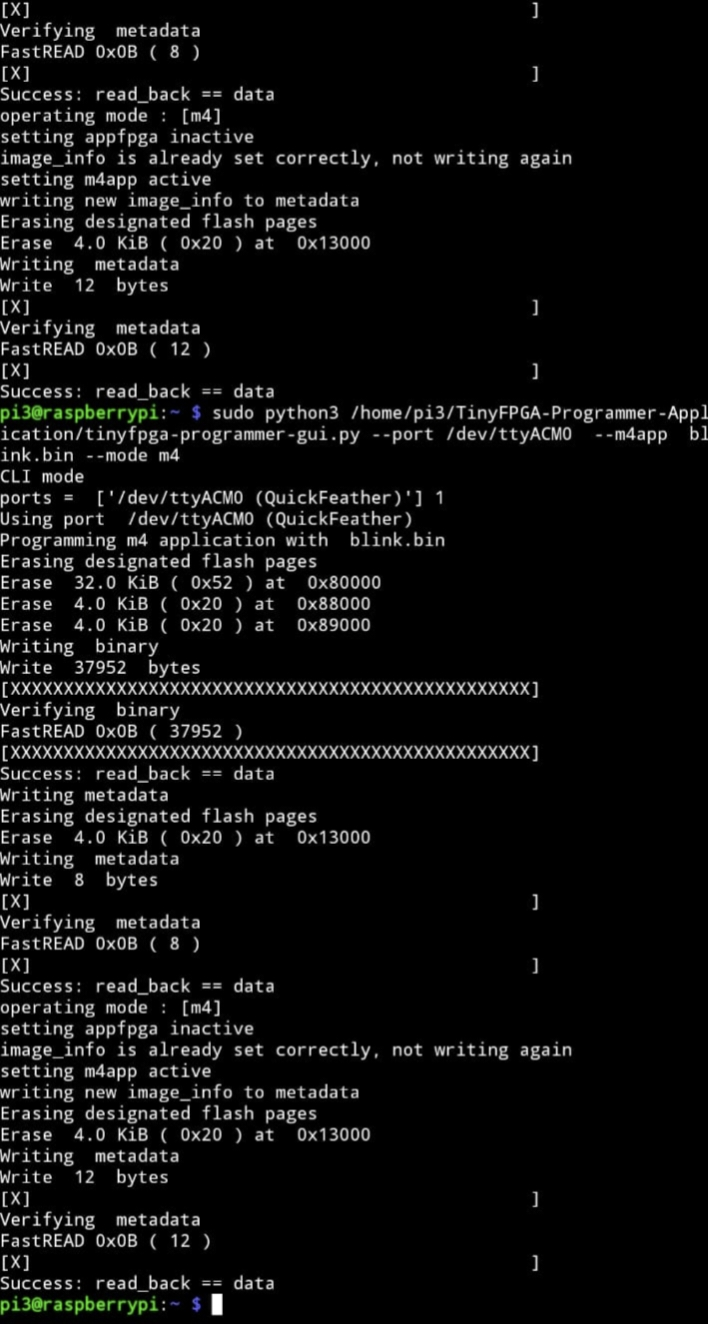
\includegraphics[width=0.3\textwidth]{ /storage/emulated/0/vignan/IMG_20241112_121251.jpg}                                
\caption{\label{fig-4:Gates}}             
\end{figure}


 \end{enumerate}

\section{RESULTS}
 \begin{enumerate}
\item Download the codes given in the link below and execute them to see the output as shown in figure 5.
\item https://github.com/BynaboyinaAiswarya/Fwc-/blob/main/Arm/main.c
 \end{enumerate}

 \begin{figure}[h]                       
\centering                               
\includegraphics[width=0.4\textwidth]{	/storage/emulated/0/vignan/IMG_20241107_154303.jpg
	 }                                
\caption{\label{fig-5:Gates}}             
\end{figure}
\section{CONCLUSION}
Hence implementation of above astract using arm code with vaman board,raspberrypi and verification through led is done .


\end{document}
